\chapter{90-Degree Contact Angle: the Physical Scenario and the Potential}

In this section, we first examine the physical conditions of a charged droplet sitting on an electrically negligible layer with a 90-degree contact angle and Reconstruct its boundary equation. Then, based on the Crowdy Map, we provide an analytical function for the entire boundary, which also serves as the equipotential lines of the scenario. Through analysis and MATLAB-based mathematical methods, we discuss the validity and application range of this function.

\section{Reconstructing the Right-Angle Case}
Consider the region $\Omega\in\mathbb{R}^2$ be the droplet of conducting fluid, surrounded by some conduct fluid and a dielectric plate. \\
...\\
\textcolor{red}{the minimization of energy for a charged conducting droplet involves the balance between electric forces and surface tension. The electric field E is generated by charges on the droplet's boundary, and the surface charge density $\sigma$ (or $\lambda$ for line charge case) is determined by the normal derivative of the potential. The energy equation is}\\
Then, we can derive the minimal energy equation:
\begin{equation}\label{minE}
    \mathcal{E} = \gamma \mathcal{P} - \frac{\epsilon_0 \epsilon_r}{2} \int_{R^2 \setminus \Omega} |E|^2 \, dS
\end{equation}

\noindent \cite{Crowdy2015} proposed that by using the first variation of energy, equation (\ref{minE}) leads to the boundary condition on the liquid-vapour interface portion of $\partial \Omega\in\mathbb{R}$ is:
\[\gamma \kappa - \frac{\lambda^2}{2 \epsilon_0 \epsilon_r} = -p\]
Here, we derive the same formula through the forces on the line $\partial \Omega$.\footnote{The way of variation method is in the appendix, some gaps are left though.
} The force due to curvature is $\gamma \int \kappa \df l$, which will be balanced by the electric force\footnote{Equation (2.50), \cite{Griffiths_2017}, pp. 103.}
\[\mathbf{f}_e=\frac{1}{2}\sigma (\mathbf{E}_{above}+\mathbf{E}_{below})\]
\noindent Since the droplet is a conductor, the interior area is an equipotential area and the electric field $\mathbf{E}_{below}$ is $0$, and $\mathbf{E}_{above}|_{\partial \Omega}=-\nabla V|_{\partial \Omega}=-\frac{\partial V}{\partial n}\hat{\mathbf{n}}$ on the boundary surface/line\footnote{On the boundary, the electric field must be perpendicular to the boundary area/line, to ensure electrons do not move on the surface of the conductor, and the interior electric field is 0.}. According to equation (\ref{ed.line}), the repulsive electrostatic force per unit line segment is
\[\mathbf{F}_e=\frac{\mathbf{E}_{above}}{2}\lambda=-\frac{1}{2}\frac{\partial V}{\partial n}\lambda\hat{\mathbf{n}}=-\frac{\lambda^2}{2\epsilon_0\epsilon_r}\hat{\mathbf{n}}\]
this is the same result as equation (4),\cite{Fontelos2008}, in $\mathbb{R}^2$. leaving the balance force equation along $\hat{\mathbf{n}}$:
\[0=\gamma\kappa\hat{\mathbf{n}}+\frac{1}{2}\lambda \mathbf{E}\]
That is:
\[0=\gamma\tilde{\kappa}+p-\frac{\lambda^2}{2\epsilon_0\epsilon_r}\]
%\subsection{First Subsection Title}

\section{Boundary Charge Density Derivation}

Given in \cite{Crowdy2015}:
\begin{equation*}
    \begin{split}
        w &= W(\zeta) = i\mu \log \zeta\\
        z &= Z(\zeta) = iA \left[ \frac{1}{\zeta} + \frac{8\zeta}{\zeta^2 - a^2} \right]\\
        \eta &= \left| \frac{dw}{dz} \right| = \left| \frac{W'(\zeta)}{Z'(\zeta)} \right| = \frac{\mu}{A} \left| \frac{\zeta^2 - a^2}{3\zeta^2 + a^2} \right|^2
    \end{split}
\end{equation*}

% Derivation of \( W'(\zeta) \)
% \[ W'(\zeta) = i\mu \frac{1}{\zeta} \]

% Derivation of \( Z'(\zeta) \) as follows:
% \begin{equation*}
%     \begin{split}
%          Z'(\zeta) &= iA \left( -\frac{1}{\zeta^2} + \frac{8(\zeta^2 - a^2) - 16\zeta^2}{(\zeta^2 - a^2)^2} \right)\\
%          &= iA \left( -\frac{1}{\zeta^2} - \frac{8(\zeta^2 + a^2)}{(\zeta^2 - a^2)^2} \right)\\
%          &= iA \frac{- (\zeta^2 - a^2)^2 - 8\zeta^2 (\zeta^2 + a^2)}{\zeta^2 (\zeta^2 - a^2)^2}\\
%          &= iA \frac{-9\zeta^4 - 6a^2\zeta^2 - a^4}{\zeta^2 (\zeta^2 - a^2)^2}\\
%          &= \frac{-iA}{\zeta^2 }\frac{(3\zeta^2 + a^2)^2}{(\zeta^2 - a^2)^2}
%     \end{split}
% \end{equation*}

% use the relation:
% \[\frac{\df w}{\df z} = \frac{\df W}{\df \zeta}\frac{\df \zeta}{\df z}=\frac{W'(\zeta)}{Z'(\zeta)}  \]

% Calculation of \(\eta\)
% \[ \eta=\left|\frac{dw}{dz}\right| = \left|\frac{W'(\zeta)}{Z'(\zeta)} \right|=\left|\frac{\mu}{\zeta}\frac{\zeta^2}{A}  \frac{(\zeta^2 - a^2)^2}{(3\zeta^2 + a^2)^2} \right|=\frac{\mu}{A}  \left|\frac{\zeta^2 - a^2}{3\zeta^2 + a^2} \right|^2\]
% as $\left|\zeta\right|=1$.
%\section{First Section Title}
\section{Study of Potential based on the Crowdy Map}
\subsection{Derivation of the Potential Function}

% \hspace{2em}Our goal is to find a conformal mapping that projects a unit circle in the $\zeta$-plane onto the entire boundary of the droplet, consisting of the upper and lower boundary, the contact line between the droplet and the substrate on which the droplet sits. As the boundary of the droplet also represents an equipotential surface, we can derive the complex potential based on the mapping. Therefore, the mapping essentially projects the geometry of a simple charge distribution to a complicated one. Applying the mapping to the simple potential function presents the potential function of the more intricate charge distribution.

% Ideally, we want to use the simplest shapes, such as a series of concentric circles in the $\zeta$-plane and project them onto the equipotential surfaces of the charged droplet in the $z$-plane. 

The original conformal mapping is given by:
\[
z = i A \left( \frac{1}{\zeta} + \frac{8\zeta}{\zeta^2 - a^2} \right)
\]
% We know that this function projects the boundary of the unit circle onto the upper boundary of the droplet. A brief exploration reveals that the arc from $-\pi/2$ to $\pi/2$ maps to the upper boundary, and the arc from $\pi/2$ to $3\pi/2$ maps to its mirror image along the y-axis.

% It is tempting to expect that the closed semicircle formed by this arc and the y-axis would project to the entire droplet boundary, yet it fails, as the $\frac{1}{\zeta}$ term obstructs and the projection function diverges at the origin. Consequently, we abandon the search for a simple closed curve inside the unit circle that maps to the entire droplet boundary.

% To ensure that the interior of the unit circle in the \( z \)-plane maps to the interior of the unit circle in the \(\zeta\)-plane, we use the following composite mapping process.

% \paragraph{Transformation Process}

% \subparagraph{2. Original Conformal Mapping:}
% Substitute \( w \) into the original conformal mapping:
% \[
% \zeta = i A \left( \frac{1}{w} + \frac{8w}{w^2 - a^2} \right)
% \]

\subsection{try find the droplet V, fail}
We expect to find a complex potential, the imaginary part of which is the potential equation of the charged droplet, parameterized by the radii of the concentric circles in the $z$-plane
\subparagraph{1. Inversion Mapping:}
\[
w = \frac{1}{z}
\]
This mapping transforms points inside the unit circle to points outside the unit circle.


Substitute \( w = \frac{1}{z} \) into the original mapping formula to obtain the new composite mapping:
% \[
% \zeta = i A \left( \frac{1}{\left(\frac{1}{z}\right)} + \frac{8\left(\frac{1}{z}\right)}{\left(\frac{1}{z}\right)^2 - a^2} \right)
% \]
% Simplify the expression:
% \[
% \zeta = i A \left( z + \frac{8z}{1 - a^2z^2} \right)
% \]
% \[
% \zeta = i A \left( \frac{9z - a^2z^3}{1 - a^2z^2} \right)
% \]

% The new composite mapping formula is:
\[
\zeta = i A \left( \frac{9z - a^2z^3}{1 - a^2z^2} \right)
\]

% \paragraph{Explanation}
% \begin{itemize}
%   \item \textbf{Step 1}: Use inversion mapping to transform points inside the unit circle to outside the unit circle.
%   \item \textbf{Step 2}: Substitute the inverted points into the original conformal mapping formula.
%   \item \textbf{Step 3}: Simplify to obtain the new composite mapping formula.
% \end{itemize}

This new formula ensures that points inside the semi-circle with its base in the \( z \)-plane map to points outside the boundary line in the \(\zeta\)-plane.

\begin{figure}[h]
\centering
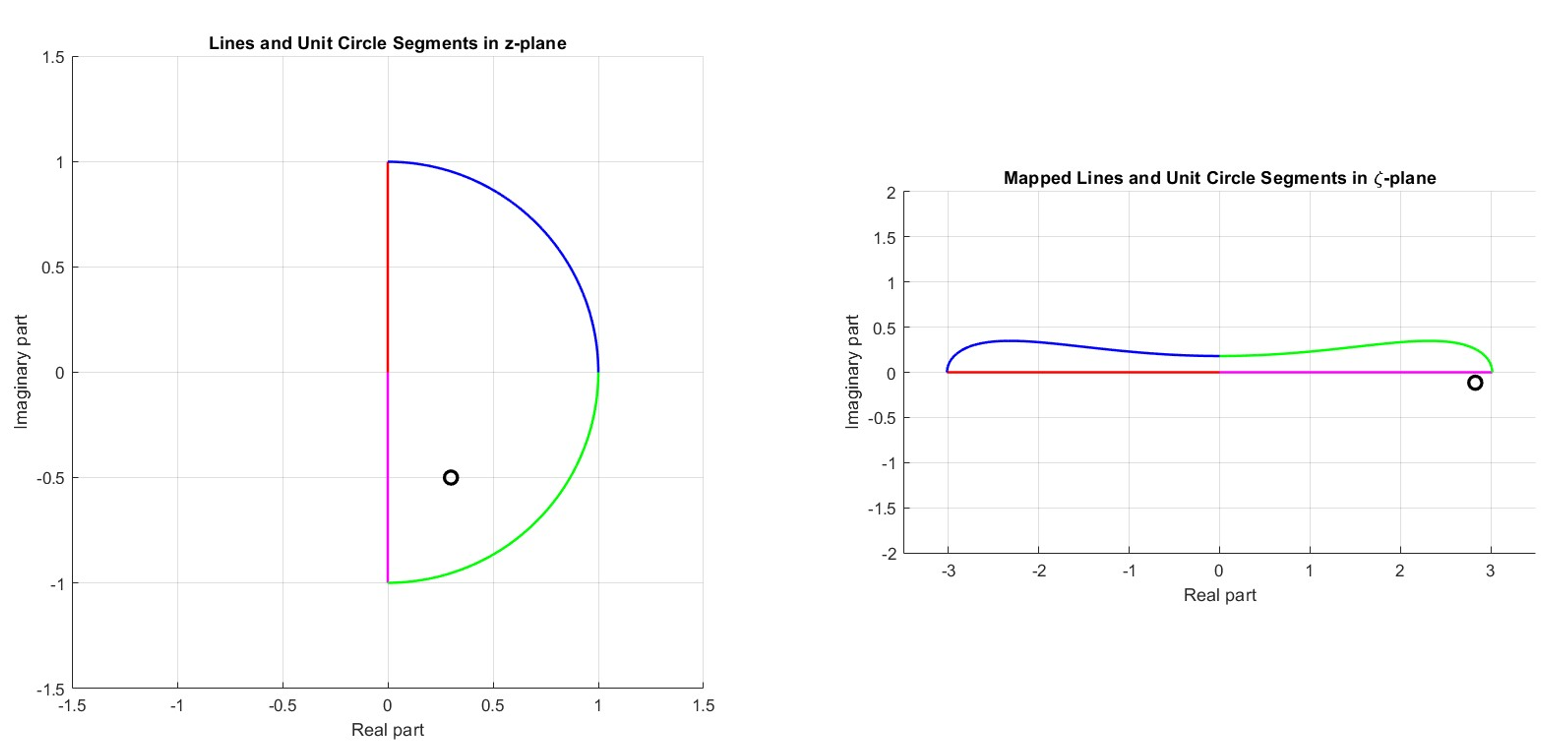
\includegraphics[width=0.75\textwidth]{Figs/crowdy2015_edit.png}
\caption{crowdy15 edit}
\label{fig:example}
\end{figure}

\subsubsection{Mapping Points Inside the Unit Circle to the Lower Half-Circle}

% Given two transformations:

% 1. Mapping points inside the unit circle to the first quadrant:
%    \[
%    \zeta_1 = \sqrt{\left( \frac{1 - \zeta}{1 + \zeta} \right) \cdot i}
%    \]

% 2. Mapping points from the first quadrant to the interior of the lower half-circle:
%    \[
%    \eta_1 = \frac{1 - \eta}{1 + \eta}
%    \]

% To find the relationship between \(\zeta\) and \(\eta\), set \(\zeta_1 = \eta_1\):
% \[
% \sqrt{\left( \frac{1 - \zeta}{1 + \zeta} \right) \cdot i} = \frac{1 - \eta}{1 + \eta}
% \]

% Multiply both sides by \((1 + \eta)\):
% \[
% \sqrt{\left( \frac{1 - \zeta}{1 + \zeta} \right) \cdot i} \cdot (1 + \eta) = 1 - \eta
% \]

% Rearrange to isolate \(\eta\):
% \[
% \sqrt{\left( \frac{1 - \zeta}{1 + \zeta} \right) \cdot i} + \sqrt{\left( \frac{1 - \zeta}{\zeta + 1} \right) \cdot i} \cdot \eta = 1 - \eta
% \]

% Combine \(\eta\) terms:
% \[
% \eta \left( \sqrt{\left( \frac{1 - \zeta}{1 + \zeta} \right) \cdot i} + 1 \right) = 1 - \sqrt{\left( \frac{1 - \zeta}{\zeta + 1} \right) \cdot i}
% \]

Solve for \(\eta\):
\[
\eta = \frac{1 - \sqrt{\left( \frac{1 - \zeta}{\zeta + 1} \right) \cdot i}}{1 + \sqrt{\left( \frac{1 - \zeta}{\zeta + 1} \right) \cdot i}}
\]

\subsubsection{Rewriting as a Hyperbolic Function}

Convert the given mapping formula into a hyperbolic function.

% Given Mapping Formula
% \[
% \eta(\zeta) = \frac{1 - \sqrt{\frac{w}{2}} - i \sqrt{\frac{w}{2}}}{1 + \sqrt{\frac{w}{2}} + i \sqrt{\frac{w}{2}}}
% \]

% where:
% \[
% w = \frac{1 - \zeta}{\zeta + 1}
% \]

% Hyperbolic Function Properties
% The definition of the hyperbolic tangent function is:
% \[
% \tanh(z) = \frac{\sinh(z)}{\cosh(z)} = \frac{e^z - e^{-z}}{e^z + e^{-z}}
% \]

% Transforming the Formula
% Considering the complex logarithm:
% \[
% \log(w) = \log \left( \frac{1 - \zeta}{\zeta + 1} \right)
% \]

% Let:
% \[
% u = \sqrt{\frac{w}{2}}
% \]

% Then the mapping formula can be rewritten as:
% \[
% \eta(\zeta) = \frac{1 - u - iu}{1 + u + iu}
% \]

% Using the Hyperbolic Tangent Function Properties
% We know:
% \[
% \tanh \left( \frac{1}{2} \log \left( \frac{1 - \zeta}{\zeta + 1} \right) \right) = \frac{\sinh \left( \frac{1}{2} \log \left( \frac{1 - \zeta}{\zeta + 1} \right) \right)}{\cosh \left( \frac{1}{2} \log \left( \frac{1 - \zeta}{\zeta + 1} \right) \right)}
% \]
This can be written as:
\[
\eta(\zeta) = \tanh \left( \frac{1}{2} \log \left( \frac{1 - \zeta}{\zeta + 1} \right) \cdot i \right)
\]

% Therefore, by using the properties of the hyperbolic tangent function, we can re-express the original mapping formula in terms of hyperbolic functions.

\subsubsection{further work, $\zeta(\eta)$}
% Square both sides to eliminate the square root:

% \[
% \frac{1 - \zeta}{\zeta + 1} \cdot i = \left( \frac{1 - \eta}{1 + \eta} \right)^2
% \]
% Expanding and rearranging terms:

% \[
% \zeta (1 + \eta)^2 - (1 + \eta)^2 = -i \zeta (1 - \eta)^2 - i (1 - \eta)^2
% \]

% \[
% \zeta (1 + 2\eta + \eta^2) - (1 + 2\eta + \eta^2) = -i \zeta (1 - 2\eta + \eta^2) - i (1 - 2\eta + \eta^2)
% \]

% Combine like terms:

% \[
% \zeta (1 + 2\eta + \eta^2 + i (1 - 2\eta + \eta^2)) = (1 + 2\eta + \eta^2 - i (1 - 2\eta + \eta^2))
% \]

% Factor out \(\zeta\):

% \[
% \zeta (1 + 2\eta + \eta^2 + i (1 - 2\eta + \eta^2)) = (1 + 2\eta + \eta^2 - i (1 - 2\eta + \eta^2))
% \]

% Finally, solving for \(\zeta\):

\[
\zeta = \frac{(1 - i) + (2 + 2i)\eta + (1 + i)\eta^2}{(1 + i) + (2 - 2i)\eta + (1 + i)\eta^2}
\]
\pagebreak
%\renewcommand\bibname{{References}}
%\bibliography{References}
%\bibliographystyle{plain}